\documentclass{beamer}
\usepackage[latin1]{inputenc}
\usetheme{Warsaw}
\title[UW Layer-1 SW Tutorial]{Layer 1 CaloTrigger Online SW Tutorial}
\author{Bucky Badger}
\institute{UW Madison}
\begin{document}

\begin{frame}
\titlepage
\end{frame}

\begin{frame}{Introduction}
\begin{itemize}
\item This document gives a rough guide to the architecture of the Layer 1 CaloTrigger Online SW
\item Outline
\begin{itemize}
\item IPBus
\item Our "soft" implementation of IPBus
\item VME and SPI byte-stream abstractions
\item Xilinx workflows
\item Existing standalone packages
\item Using XMD to upload and debug SW
\item ToDo list
\end{itemize}
\end{itemize}
\end{frame}

\begin{frame}{IPBus}
\begin{itemize}
\item Common CMS protocol for interacting with Trigger HW
\item Basically a specification for interpreting a byte stream to:
\begin{itemize}
\item READ $n$ words (32-bit) from an address in device memory 
\item WRITE $n$ words (32-bit) into an address
\item READ-WRITE-MODIFY at word at an address
\end{itemize}
\item Below: the specification for a READ request/response
\end{itemize}
\begin{center}
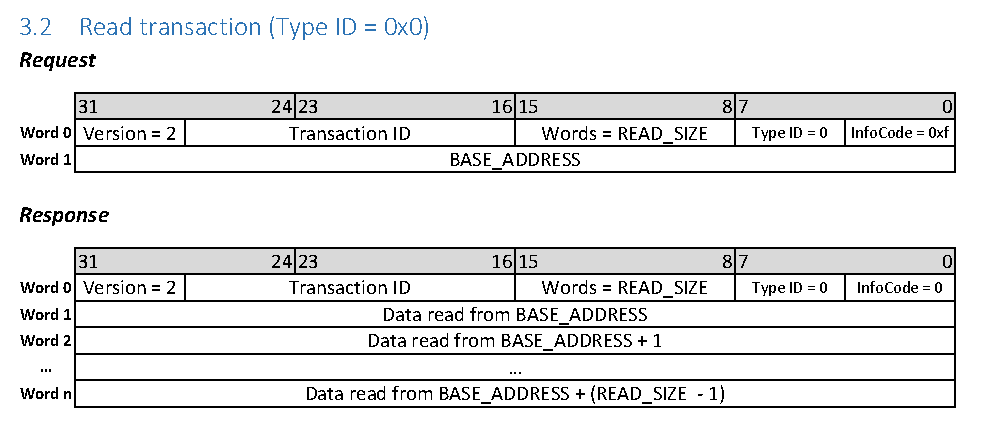
\includegraphics[width=0.8\textwidth]{images/ipbus_read.pdf}
\end{center}

\end{frame}


\end{document}
